\documentclass[a4paper,12pt]{article}
\usepackage[left=1.0in, right=1.0in, top=0.5in, bottom=0.8in]{geometry}
\usepackage[utf8]{inputenc}
\usepackage[T1]{fontenc}
\usepackage[english]{babel}
\usepackage{amsmath,amssymb,amsthm,amsfonts}
\usepackage{float}
\usepackage{graphicx}
\usepackage{caption}
\usepackage{subcaption}

\title{
	Assignment 1\\
	EL2700 Model Predictive Control
}
\author{
	Kartik Chari\\
	kartikc@kth.se\\
	960807-0174
	\and
	Saurabh Vyas\\
	saurabhv@kth.se\\
	970202-T198
}

\begin{document}
\maketitle

\section{Analytical Task}
Let $x_1$ = $\theta$, $x_2$ = $\dot{\theta}$ and  cart acceleration u = $\dfrac{F}{M}$ \\
$\therefore$ The dynamics of the inverted pendulum is given as:

\begin{equation}
\begin{bmatrix}
  \dot{x_1} \\
 \dot{x_2}
\end{bmatrix}
=\begin{bmatrix}
 x_2\\
-a_0 sin(x_1) - a_1 x_2\\
\end{bmatrix}
+\begin{bmatrix}
0\\
b_0 u cos(x_1)\\
\end{bmatrix} \ \ ; \ y = x1
\label{invPend}
\end{equation}

$\forall \ a_0 = - \dfrac{mgl}{I + ml^{2}} \ , \ a_1 = \dfrac{b_p}{I + ml^{2}} \ and \ b_0 = \dfrac{ml}{I + ml^{2}}$
	\subsection{Equilibrium Point}
	In order to find the equilibrium point, set the external inputs and the time derivatives of the states to 0. $\implies$ $u = 0 ; \ \dot{x_1} = 0 ; \ \dot{x_2} = 0 ;$
	Thus, we get 
	\begin{align*}
	x_2 &= 0 \\
	sin(x_1) &= 0
	\end{align*}
This means that the equilibrium points can be (n$\pi$, 0). But as we are studying inverted pendulum dynamics, the acceptable equilibrium points are (2n$\pi$, 0). \\
Thus, the upright pendulum position at rest, $x\textsubscript{ref} = [0, \ 0]^{T}$ is the equilibrium point for equation (\ref{invPend}).

	\subsection{Linearization}
	In order to linearize the Nonlinear dynamics of equation (\ref{invPend}),  \textit{Taylor Series of Expansion} was used to obtain the following Jacobian matrices:
	\begin{equation}	 
		J_x = \begin{bmatrix}
			\dfrac{\partial f_1}{\partial x_1} \biggr \vert_{X_{ref} = 0,U_{ref} = 0} & \dfrac{\partial f_1}{\partial x_2} \biggr \vert_{X_{ref} = 0,U_{ref} = 0}\\ \\
			\dfrac{\partial f_2}{\partial x_1} \biggr \vert_{X_{ref} = 0,U_{ref} = 0} & \dfrac{\partial f_2}{\partial x_2} \biggr \vert_{X_{ref} = 0,U_{ref} = 0}
		\end{bmatrix}
		= \begin{bmatrix}
			0 & 1 \\
			-a_0 & -a_1
		\end{bmatrix}
	\label{stJcb}
	\end{equation}
	
	\begin{equation}
		J_u = \begin{bmatrix}
			\dfrac{\partial f_1}{\partial u} \biggr \vert_{X_{ref} = 0,U_{ref} = 0} \\ \\
			\dfrac{\partial f_2}{\partial u} \biggr \vert_{X_{ref} = 0,U_{ref} = 0} 
		\end{bmatrix}
		= \begin{bmatrix}
			0  \\
			b_0
		\end{bmatrix}
	\label{inpJcb}
	\end{equation}
	
	$\forall$ $f_1 \ = \ \dot{x_1}$ and $f_2 \ = \ \dot{x_2}$ \\
	
Thus, from eq (\ref{stJcb}) and (\ref{inpJcb}), we get the linearized continuous-time system as follows :
	\begin{equation}
	\boxed{
		\begin{bmatrix}
  			\Delta \dot{x_1}(t) \\
			 \Delta \dot{x_2}(t)
		\end{bmatrix}
		=\begin{bmatrix}
 			0 & 1\\
			-a_0 & - a_1\\
		\end{bmatrix}
		\begin{bmatrix}
			\Delta x_1 (t) \\
			\Delta x_2 (t)
		\end{bmatrix}
		+\begin{bmatrix}
			0\\
			b_0 
		\end{bmatrix}
		u \  \ ; \
		\Delta y(t) = \begin{bmatrix}
			1 & 0
		\end{bmatrix}
		\begin{bmatrix}
			\Delta x_1 (t) \\
			\Delta x_2 (t)
		\end{bmatrix} }
\label{linCont}
	\end{equation}
	$\forall$ $\Delta x_1(t) \ = \ x - x_{ref}$, $\Delta u(t) \ = \ u - u_{ref}$ and $\Delta y(t) \ = \ y - C_c \ x_{ref}$ \\
Thus, from the above equation (\ref{linCont}), we can extract the following required matrices:
	\begin{equation}
	\boxed{
		A_c = \begin{bmatrix}
			0 & 1\\
			-a_0 & - a_1\\
		\end{bmatrix}
	\ ; \ B_c = \begin{bmatrix}
			0\\
			b_0
		\end{bmatrix}
	\ ; \ C_c = \begin{bmatrix}
			1 & 0
		\end{bmatrix}}
	\end{equation}
	
	\subsection{Zero Order Hold Discretization}
	The general form of the Discrete time linear system is as follows:
	\begin{equation}
\begin{cases}
		x_{t+1} &= A x_t + B u_t \\
		y_t &= C x_t \\
	\end{cases}
	\label{linDisc}
\end{equation}
The discrete-time matrices \textbf{A},\textbf{B},\textbf{C} are obtained by solving the continuous-time system in equation (\ref{linCont}) for state x at times th and (t+1)h as follows:
\begin{align*}
A &= e^{A_c h} \\
B &= \int_{0}^{h} e^{A_c s} B \ ds \\
C &= \ same \ as \ C_c
\end{align*}
$\therefore$ Let \textit{h} be the Sampling Period \\
\textbf{METHOD 1}:
\begin{align*}
A &= e^{A_c h} \\
&= e^{\begin{bmatrix}
	0 & h\\
	-a_0 h & - a_1 h\\
\end{bmatrix}}
\end{align*}
Now, using the Maclaurin Series of Expansion for $e^{x}$, we get
\begin{align*}
	e^{x} &= 1 + \dfrac{x}{1!} + \dfrac{x^2}{2!} + \dfrac{x^3}{3!} +... \\ 
\end{align*}
Thus, for the ease of calculation, we ignored the Higher Order Terms and derived the Discrete-time System matrix as follows:
\begin{align*}
	e^{A_c h} &= I + \begin{bmatrix}
		0 & h\\
		-a_0 h & - a_1 h\\
	\end{bmatrix} 
\end{align*}
\begin{equation}
\therefore
\boxed{
	A = \begin{bmatrix}
		1 & h\\
		-a_0 h & 1 - a_1 h\\
\end{bmatrix}}
\end{equation}
Now, for deriving B, we need to calculate the Particular integral 
\begin{align*}
	B &= \int_{0}^{h} e^{A_c s} B \ ds \\
	&= \int_{0}^{h} \begin{bmatrix}
			1 & s\\
			-a_0 s & 1 - a_1 s
	\end{bmatrix} 
	\begin{bmatrix}
		0\\
		b_0\\
	\end{bmatrix} ds \\
	&= \int_{0}^{h} \begin{bmatrix}
			s \ b_0\\
			(1 - a_1 s) b_0
	\end{bmatrix} ds
\end{align*}
$\therefore$
\begin{equation}
\boxed{
B = \begin{bmatrix}
b_0 \ \dfrac{h^2}{2} \\ \\
b_0 h \ - \ \dfrac{a_1 b_0 h^2}{2}
\end{bmatrix}}
\end{equation}
Also, the C matrix remains the same.
\begin{equation}
\boxed{
C = \begin{bmatrix}
1 & 0
\end{bmatrix}}
\end{equation}

\textbf{METHOD 2}:
\begin{align*}
A &= e^{A_c h} \\
&= e^{\begin{bmatrix}
	0 & h\\
	-a_0 h & - a_1 h\\
\end{bmatrix}}
\end{align*}
Using the definition of State Transition Matrix, we get
\begin{align*}
e^{A_c t} &=  \mathcal{L}^{-1} \{ [sI - A_c]^{-1}\} \\ \\
&= \mathcal{L}^{-1} \{[\begin{bmatrix}
s & 0 \\
0 & s
\end{bmatrix}
- \begin{bmatrix}
0 & h\\
-a_0 h & - a_1 h\\
\end{bmatrix}]^{-1}
\} \\ \\
&= \mathcal{L}^{-1} \{[\begin{bmatrix}
\dfrac{s + a_1}{s^2 + a_1 s + a_0} & \dfrac{1}{s^2 + a_1 s + a_0} \\ \\
\dfrac{-a_0}{s^2 + a_1 s + a_0} & \dfrac{s}{s^2 + a_1 s + a_0}
\end{bmatrix}] \}
\end{align*}
Now, from Laplace Inverse Table, we have 
\begin{align}
\mathcal{L}^{-1} \{\dfrac{(s+a)}{(s+a)^2- b^2} \} &= cosh(bt)*e^{-at}
\label{eq1}
\end{align}
\begin{align}
\mathcal{L}^{-1} \{\dfrac{b}{(s+a)^2- b^2} \} &= sinh(bt)*e^{-at}
\label{eq2}
\end{align}
$\therefore$ Assuming \textit{$q = \dfrac{a_1}{2}$} and \textit{$p = \dfrac{\sqrt{a_1^2 - 4a_0}}{2}$} and using eq(\ref{eq1}) and eq(\ref{eq2}) to solve the above expression, we get
\begin{figure}[H]
\centering
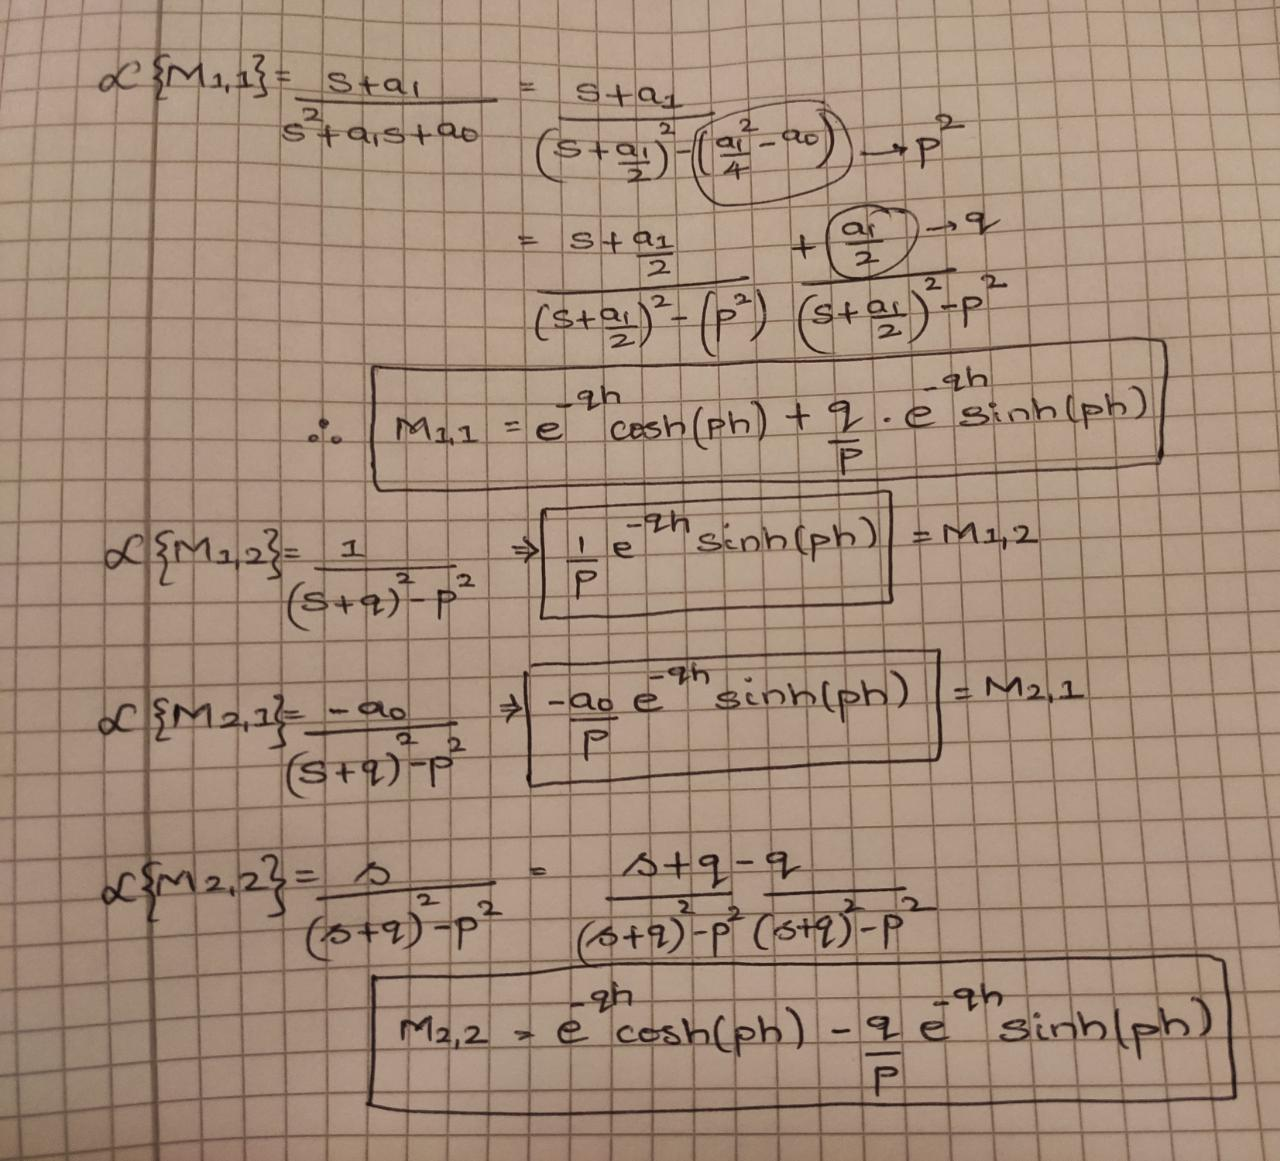
\includegraphics[scale=0.4]{image_1.jpeg}
\caption{\textbf{Steps for the Laplace Inverse Calculation}}
\label{A_cal}
\end{figure}
\begin{equation}
\implies
\boxed{
A = \begin{bmatrix}
e^{-qh}*cosh(ph) + \dfrac{q}{p}e^{-qh}*sinh(ph) & \dfrac{1}{p}*e^{-qh}*sinh(ph) \\
\dfrac{-a_0}{p}e^{-qh}*sinh(ph) & e^{-qh}*cosh(ph) - \dfrac{q}{p}e^{-qh}*sinh(ph)
\end{bmatrix}}
\end{equation}
Now, for deriving B, we need to calculate the Particular integral 
\begin{align*}
	B &= \int_{0}^{h} e^{A_c s} B \ ds \\
	&= \int_{0}^{h} \begin{bmatrix}
	e^{-qs}*cosh(ps) + \dfrac{q}{p}e^{-qs}*sinh(ps) & \dfrac{1}{p}*e^{-qs}*sinh(ps) \\
\dfrac{-a_0}{p}e^{-qs}*sinh(ps) & e^{-qs}*cosh(ps) - \dfrac{q}{p}e^{-qs}*sinh(ps)
	\end{bmatrix} \begin{bmatrix}
	0 \\
	b_0
	\end{bmatrix} ds \\ \\
	&= \int_{0}^{h} \begin{bmatrix}
	\dfrac{b_0}{p}*e^{-qs}*sinh(ps) \\
	b_0e^{-qs}*cosh(ps) - b_0\dfrac{q}{p}e^{-qs}*sinh(ps)
	\end{bmatrix} ds
\end{align*}
\begin{figure}[H]
\centering
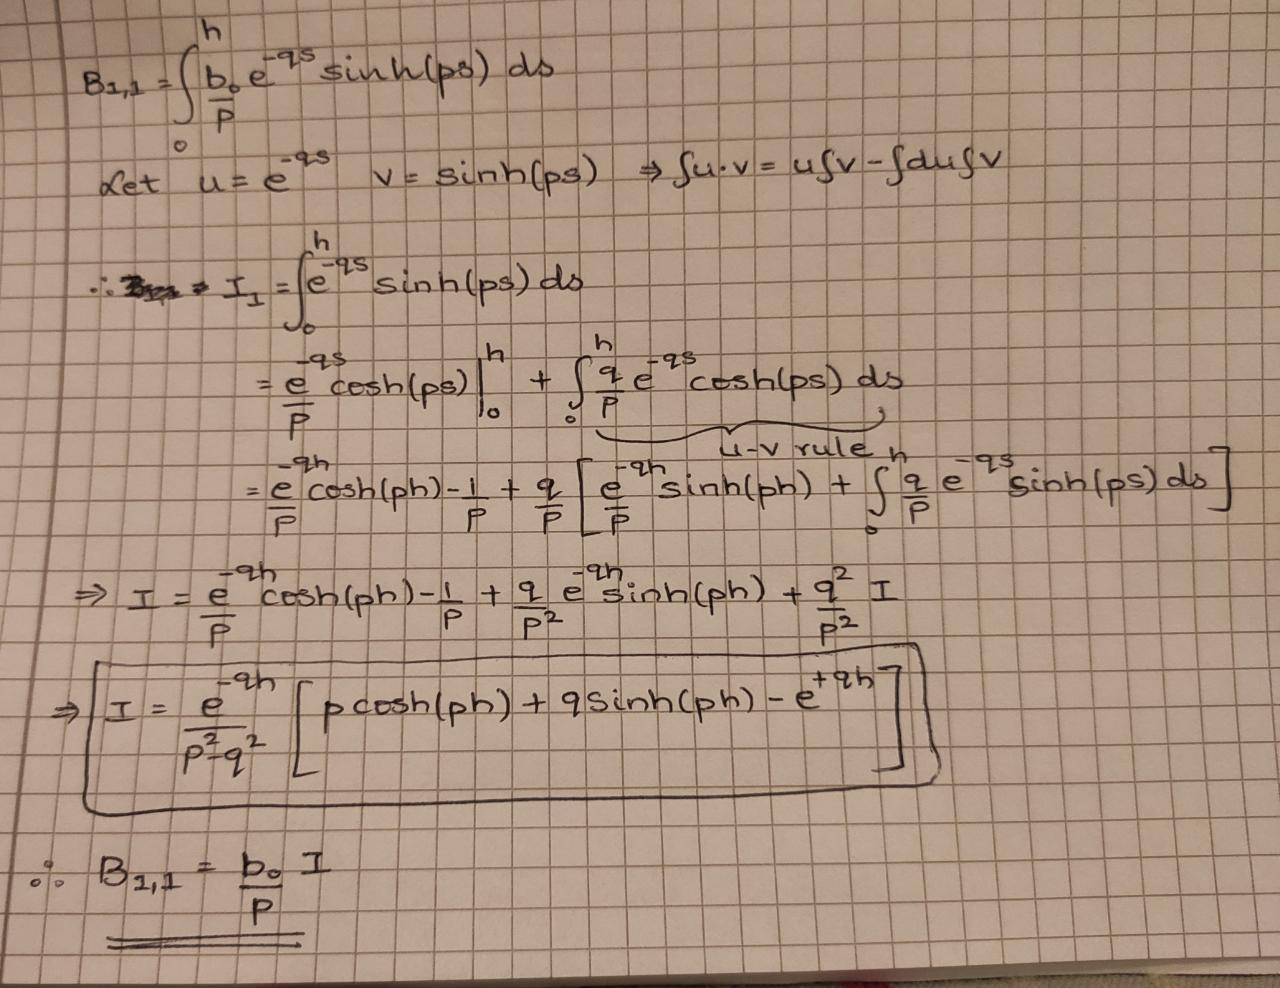
\includegraphics[scale=0.4]{image_2.jpeg}
\caption{\textbf{Steps for the B Matrix Calculation}}
\label{B_cal}
\end{figure}
Similarly if we solve for $B_{2,1}$, we get the following B matrix
\begin{equation}
\boxed{
B = \begin{bmatrix}
\dfrac{b_0}{p}[\dfrac{e^{-qh}}{p^2-q^2}(p*cosh(ph)+q*sinh(ph)-e^{qh})] \\ \\
\dfrac{b_0 e^{-qh}}{p^2-q^2}\{(p*sinh(ph)+q*cosh(ph)-q*e^{qh}) - \dfrac{q}{p}(p*cosh(ph)+q*sinh(ph)-e^{qh})\}
\end{bmatrix}}
\end{equation}
And, \begin{equation}
\boxed{
C = \begin{bmatrix}
1 & 0
\end{bmatrix}
}
\end{equation}
	\subsection{Impact of Sampling on Pole locations}

		\subsubsection{Effect of changing h on Discrete-time poles}
		Here, the numerical values from the Part II data have been used to evaluate the effect of changing the Sampling interval(h) from 0.01 to 0.7 with increments of 0.01 as follows:
	\begin{figure}[H]
	\centering
	\begin{subfigure}[b]{0.5\textwidth}
	    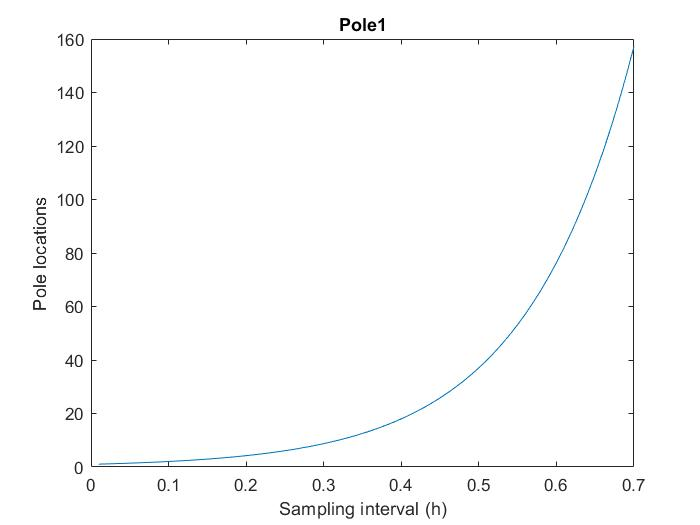
\includegraphics[width=\textwidth]{Design_Task_1/h_pole1.jpg}
	    \caption{\textit{Effect on first pole}}
	    \end{subfigure}
	    \vspace{1em}
	    \begin{subfigure}[b]{0.5\textwidth}
	    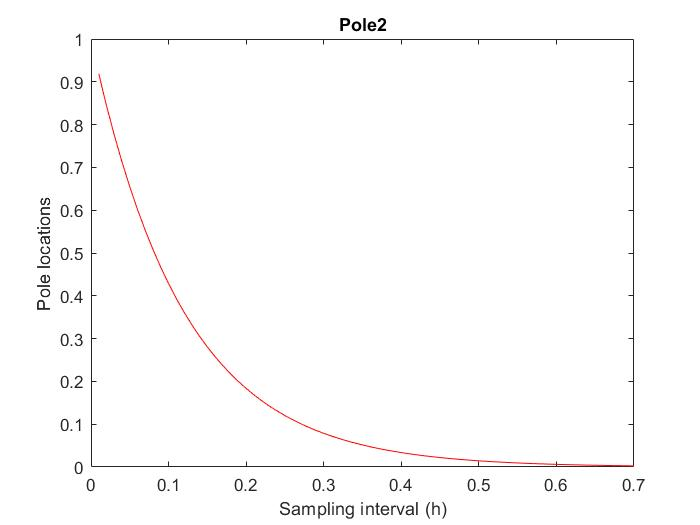
\includegraphics[width=\textwidth]{Design_Task_1/h_pole2.jpg}
	    \caption{\textit{Effect on Second Pole}}
	    \end{subfigure}
	    \caption{\textbf{Plot of effect of changing \textit{h} on Discrete-time poles}}
	    \label{fig1}
	\end{figure}

The above sub-figure(\ref{fig1}a) shows the change in the first discrete eigen- value as the sampling interval is increased and the sub-figure(\ref{fig1}b) shows the corresponding change in the second discrete eigen value. \\
	Thus, we observe that as \textit{h} is increased, the first pole of the discrete-time system slowly moves towards the unit circle and on further increasing \textit{h}, it shoots out exponentially; thereby, destabilizing the system. 
	On the other hand, the second pole exponentially moves away from the unit circle towards the origin. \\
	The above observations can be easily verified by the mapping relation $Z_i \ = \ e^{S_i*h}$ as shown in the next subsection. 


	\subsubsection{Relationship between Continuous-time and Discrete-time Poles}	
	Let \textit{$S_i$} denote the continuous time poles and \textit{$Z_i$} denote the discrete time poles. \\
	\begin{figure}[H]
	\centering
	\begin{subfigure}[b]{0.5\textwidth}
	    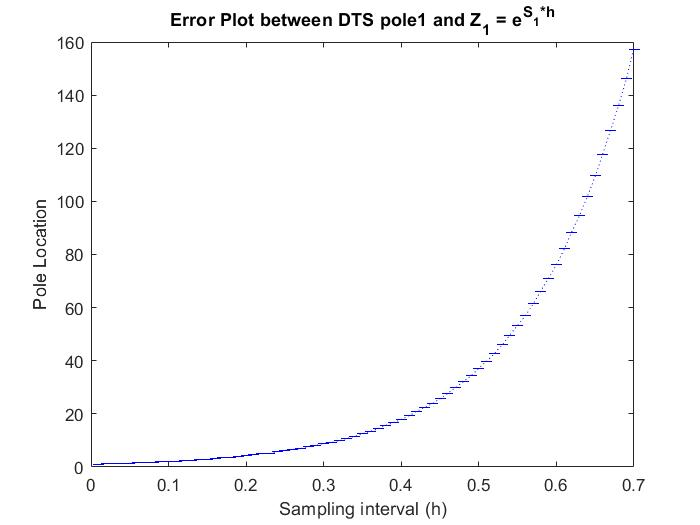
\includegraphics[width=\textwidth]{Design_Task_1/errplot1.jpg}
	    \caption{\textit{Errorplot of the first pole}}
	    \end{subfigure}
	    \vspace{1em}
	    \begin{subfigure}[b]{0.5\textwidth}
	    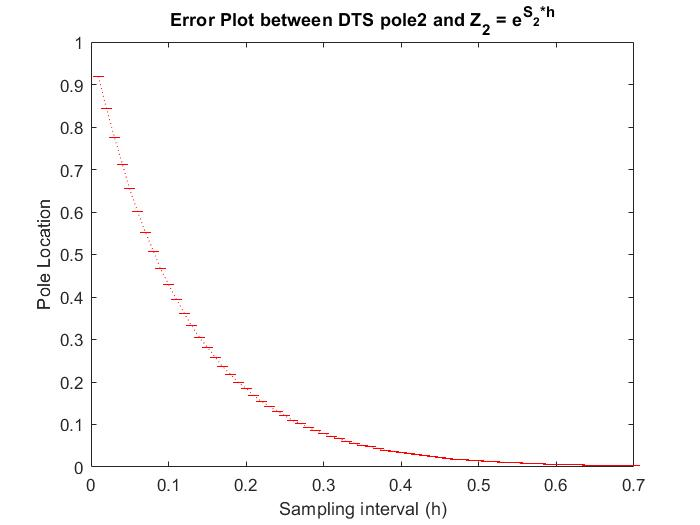
\includegraphics[width=\textwidth]{Design_Task_1/errplot2.jpg}
	    \caption{\textit{Errorplot of the second Pole}}
	    \end{subfigure}
	    \caption{\textbf{Verification of the mapping between Continuous-time poles and Discrete-time poles}}
	    \label{fig2}
	\end{figure}
	Thus, the mapping between the Continuous-time and Discrete-time ($Z_i \ = \ e^{S_i*h}$) is verified using the \textit{errorbar} plot in MATLAB(see fig(\ref{fig2})).
	\section{Design Task}
	In this part a state feedback controller is designed and tested with the nonlinear inverted pendulum model using Simulink.
	\subsection{Design of State Feedback Controller}
	The MATLAB script for defining the model dynamics is filled with A,B,C and D matrix. In order to achieve the design targets, the desired pole locations are \textit{placed} closer to the unit circle. The state feedback gain L is computed using the place function and the feed-forward gain \textit{$l_r$} is computed with the help of it.
	\begin{figure}[H]
	\centering
	\begin{subfigure}[b]{0.75\textwidth}
	    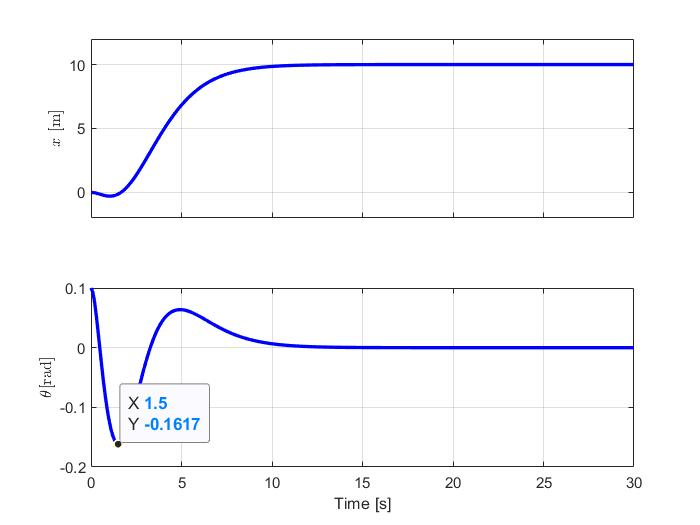
\includegraphics[width=\textwidth]{Design_Task_1/plot3.jpg}
	    \caption{\textit{Cart position and pendulum angle plot}}
	    \end{subfigure}
	    \vspace{1em}
	    \begin{subfigure}[b]{0.75\textwidth}
	    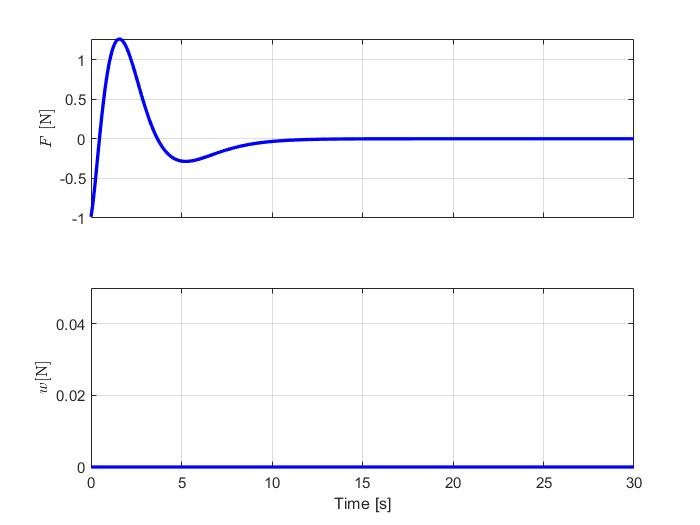
\includegraphics[width=\textwidth]{Design_Task_1/plot4.jpg}
	    \caption{\textit{Force and disturbance plot}}
	    \end{subfigure}
	    \caption{\textbf{Results for controller without disturbance}}
	    \label{fig2.1}
	\end{figure}	
	Fig(\ref{fig2.1}) shows the results for the controller without any disturbances. It can be seen that the design targets are met since the maximum angle of the pendulum is under 10 degrees and the cart reaches 9 meters before 10 seconds. \\
	\subsection{Performance in presence of disturbance input}
	A small disturbance is introduced in the simulation in order to evaluate the controller robustness. 
	\begin{figure}[H]
	\centering
	\begin{subfigure}[b]{0.75\textwidth}
	    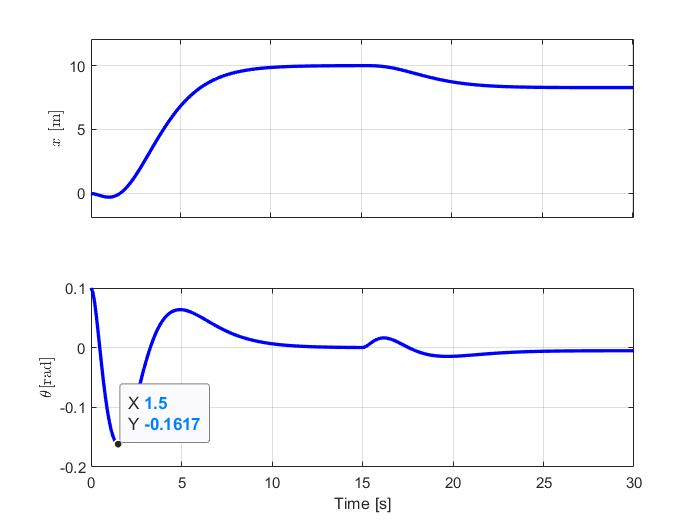
\includegraphics[width=\textwidth]{Design_Task_1/plot5.jpg}
	    \caption{\textit{Cart position and pendulum angle plot}}
	    \end{subfigure}
	    \vspace{1em}
	    \begin{subfigure}[b]{0.75\textwidth}
	    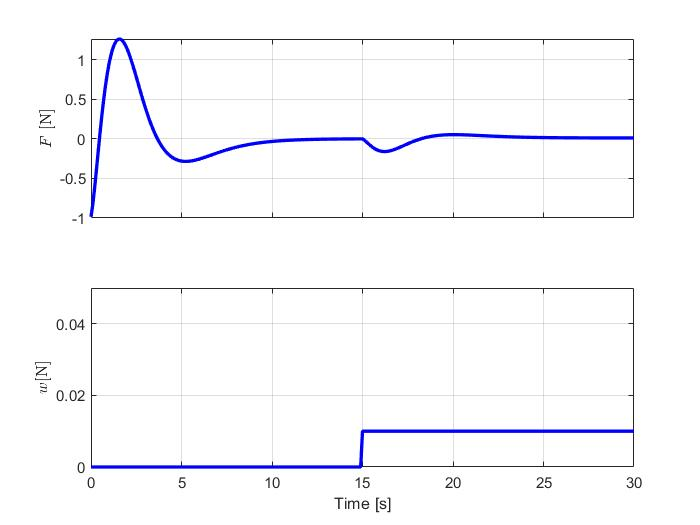
\includegraphics[width=\textwidth]{Design_Task_1/plot6.jpg}
	    \caption{\textit{Force and disturbance plot}}
	    \end{subfigure}
	    \caption{\textbf{Results for controller without disturbance}}
	    \label{fig2.2}
	\end{figure}
	From Fig(\ref{fig2.2}) it can be seen that when a small disturbance is introduced, the controller keeps the system stable and brings the pendulum back to its equilibrium position. However, the cart position is changed by a small amount resulting in a steady state error which can be verified by 
	\begin{equation}
    y_{ss} = -C[I - (A - BL)]^{-1} B_w w
    \end{equation}
\end{document}